\documentclass{sig-alternate}

\usepackage{graphicx}
\usepackage{url}
\usepackage{hyperref}
\hypersetup{breaklinks}
\linespread{1.6}

\begin{document}
\title{Social WiFi Authentication}
\author{Ross Nordstrom\\
        University of Colorado - Colorado Springs\\
        1420 Austin Bluffs Pkwy,\\
        Colorado Springs, CO 80918\\
        \texttt{rnordstr@uccs.edu}
       }
\date{December 2014}

\maketitle

\begin{abstract}
Wireless network authentication techniques have been greatly studied and improved over the past two
decades, but they all suffer from the human factor. A common problem in computer and network
security is ensuring the people interacting with it do not introduce security holes. Residential
and small business networks are an example of an area where security is very important but not well
understood. The simple fact is that the algorithm keeping wireless networks is of no use if the
network owner uses insecure passwords, or insecure practices in keeping those passwords a secret.

In this paper I investigate the use of OAuth for authenticating and managing authorization of
wireless networks. By using OAuth, we can frame the authentication scheme to match users' mental
model of access control. OAuth, through integration with Google+ or Facebook, let's network owners
manage access to their network more intuitively by simplifying the concept to a matter of managing
a list of people in a group. In addition to improving access control, authenticating with OAuth
removes the need for passwords and the insecurities introduced from them in residential and small
business wireless networks.
\end{abstract}

\category{D.4.6}{Security and Protection}{Authentication}
\terms{Security}
\keywords{Security, Authentication, OAuth, Wifi, Wi-Fi, Cloud}

\section{Introduction}
\label{section:introduction}
In this paper I present the existing methods of authentication for Wireless networks (specifically
WLANs). In general, they fall into two categories targeting (1) Residential and Small Office
networks and (2) Enterprise networks. While each suffers for different reasons, I propose both would
benefit from integration with OAuth providers such as Google, Facebook, Github, Twitter, or a
private OAuth server. Offloading authentication to these providers contributes to both small and
enterprise networks in different ways, while improving the user experience in both cases.

\subsection{Residential and Small Networks}
The first type of network suffers heavily from lack of understanding of wireless networks and
``the human factor,'' which introduces vulnerabilities not inherent to the authentication protocol.
In these networks, there are likely to be relatively few users, each with relatively many devices.
Most of these devices will already be authenticated to social OAuth providers, which would allow
for wireless network authentication software to prompt the user to simply reuse that authentication
for access to the WLAN.

These small networks are the primary target of this proposal, as they stand to gain the most through
the ease of use introduced by socially-authenticated WLANs.

\subsection{Enterprise Networks}
The second type of network would benefit from integration with OAuth providers because it would
offload maintenance of yet another server(s). Additionally, more and more enterprises are using
OAuth for internal authentication, so this would allow them to reuse their main authentication
mechanism \cite{todo:OAuthEnterprise}.
\section{Motivation}
\label{section:motivation}
Existing WiFi authentication mechanisms, while technically secure, tend to create a poor user
experience and become vulnerable because of unpredictable behaviors of the users. Additionally,
most methods of authentication make it difficult for an administrator to revoke access to the
network, or even see who and what has access to begin with.

\subsection{Authentication Types}
There are several authentication techniques supported for communication over WiFi. They include
the following types of authentication, roughly in ascending order of security: \cite{WifiAuthenticationTypes}
\begin{description}
  \item{Open Authentication:} Devices must have a Wired Equivalent Privacy (WEP) key matching the access point's WEP keys.
  \item{Shared Key Authentication:} Similarly, devices have a shared key. The access point sends an unencrypted challenge text to the device, who responds with the same text encrypted with the shared key.
  \item{MAC Address Authentication:} An access point can be configured with a white-list of allowed device MAC addresses. Any device with a MAC address on that list can communicate over the network.
  \item{EAP Authentication:} The Extensible Authentication Protocol (EAP) defines a set of interactions between the device and a RADIUS server, with the access point relaying. Once authenticated, the device gets a unique WEP key for continued authenticated access.
  \item{WPA Authentication:} Wi-Fi Protected Access has devices authenticate much like EAP, with some differences in key management.
\end{description}

\subsection{Shared Keys}
WiFi authentication typically works based on the sharing of an SSID and a secret or password.
This works, and allows for secure communication between a device who has the SSID/secret and
the wireless router or access point. The challenge with this shared secret technique is it
can be tedious to share with users. Additionally, to improve the security of a shared secret,
it should be (1) hard to guess and therefore a mixture of alphanumeric and special characters,
(2) hard to brute force and therefore long enough to challenge current and (near-) future computers,
and (3) is changed regularly reducing the window of opportunity intruders have on the network.



\subsection{Some Subsection}
[subsection here]

\section{Related Work}
\label{section:relatedwork}

TODO: Coova....
\section{Proposed Design}
\label{section:propeseddesign}
I propose instrumenting a wireless network to enforce authorization through integration with an
OAuth provider (Facebook). I will prototype a simple authorization scheme to allow the network
owner's friends access to the network. To create the authentication and authorization flow, I will
program a dual-band OpenWRT router to have an open SSID with a captive portal where the user will
use OAuth with Facebook to prove to the router who they are. At setup time, the network owner will
integrate the router with their list of Facebook friends. As users present themselves to the router,
if they are found to be in the owner's list of friends, they will be presented temporary credentials
to the second, WPA-encrypted SSID. Rather than take on the challenge of creating per-user keys on
the encrypted SSID, I will simply automate the resetting of the key to some frequent interval, such
as 1-2 times a day.

While my initial prototype will be fairly manual, it is meant to be a proof of concept. Should this
idea prove itself, my proposal is to publish the implementation as open-source router firmware and
open-source client apps/services to automate the handshaking. By open-sourcing the implementation,
router manufacturers could include the software in their products and device OS's could be modified
to implement the client-side automation.

\subsection{Handshaking}
Here, I detail the steps and actions taken by the network owner, user(s), and instrumented router to
achieve OAuth-secured wireless network.

\begin{description}
\item{Setup:} First, the network owner will authenticate the router on her behalf with Facebook,
granting it access to her list of friends. The router will store the resulting server access token
so it can periodically query Facebook in order to update the list of friends. This list will include
an identifier for each friend.

The owner will then setup two SSIDs: an open SSID with a captive portal requesting users to
authenticate with Facebook, and a WPA-encrypted SSID with full network access.

\item{Access Request:} Users will connect to the open SSID and complete an OAuth authentication with
Facebook, granting the captive portal server some basic information about them, including an
identifier. If the user declines or fails to complete the OAuth request, they will be denied.

\item{Access Authorization:} The captive portal server will search for the user's identifier in the
network owner's list of friends. If found, the captive portal will continue with an Access Response.

\item{Access Response:} The captive portal will then response with the credentials needed for the
encrypted SSID.

\item{Switch to Secure SSID:} Initially the user will need to manually switch over to the encrypted
SSID and enter the credentials provided in the \texttt{Access Response} step. Eventually this flow
would be automated by instrumenting the client, such as an Android service.
\end{description}
\section{Implementation}
\label{section:implementation}
Given the scope of this project, I aimed to achieve a minimum viable prototype, leaving improvements
to get it actually adopted for Future Work\ref{section:futurework}.

\subsection{Proof of Concept Goals}
Here I break down the work I did to create an initial proof of concept. Note that all captive portal
communication would eventually be over SSL/TLS to ensure the credentials eventually passed to the
user cannot be read by eavesdroppers.

\subsubsection{Captive Portal}
The first thing I need to do is implement a captive portal on an OpenWRT router, where I can
redirect all users of the open SSID to an authentication page.

\subsubsection{Router-Facebook Integration}
The next thing I need to do is integrate the router with Facebook and authenticate it on behalf of
the owner in order to get a list of their friends. Additionally I need to securely store the OAuth
token allowing the router to authenticate for the owner to Facebook.

\subsubsection{User-Facebook Authentication}
The next step is to have users authenticate with Facebook so the captive portal server can learn
their identity and see if they are one of the owner's friends. If they are found to be in that list,
the server will present the user with the credentials to the secure SSID.

\subsubsection{Programmatic SSID Re-keying}
The final step in the proof of concept is to show that I can program the router to periodically
change the access credentials for the encrypted SSID.

\subsection{Proof of Concept Implementation}
It turns out there's an open source tool for instrumenting an OpenWRT router with a captive portal
and RADIUS. The product is CoovaAP \cite{product:CoovaAP}, and it can be deployed as a simple
firmware upgrade to OpenWRT-enabled routers. Specifically I worked with a Linksys WRT54GL
\cite{product:WRT54GL}.

An interesting and extremely relevant feature of CoovaAP is support for ``Facebook HotSpot Captive
Portal.'' Unfortunately, it has not been maintained and has not worked in several years
\cite{article:CoovaFacebookDead}. In lieu of this, I decided to try out integrating with Google+
OAuth as a proof of concepts. Luckily, CoovaAp support programming a HotSpot server, so I tried
instrumenting this. I was able to setup a Google Project with which to authenticate, but could not
get the Hotspot server to integrate with it in the time I had. Details on the code I wrote and
setup I did can be found in the appendix \ref{section:appendix}. Many of the challenges I faced
had to do with the documentation for using CoovaAp. In many cases, the documentation was outdated,
in other cases there simply wasn't the level of detail I could have used to improve my setup time.

\section{Future Work}
\label{section:futurework}
Future work on my idea will mainly take more time in order to complete a proof of concept
demonstrating OAuth-based access to a wifi network. Since it's already been done with CoovaAp, the
major focus should be on ease of use, supporting several providers, and marketing the idea rather
than ability to do the authentication.

\subsection{Ease of Use}
Just as the original goal of my research was to improve security of WiFi networks by making it easy
for non-tech-savvy users to maintain secure networks, future work should respect this primary goal.
Ease of use of the system falls into two categories: (1) ease of setting up and maintaining the
networks, and (2) ease of authenticating to the network with a minimum of work

With the prevalence social authentication on users' devices, it should be feasible to reuse existing
authenticated sessions with identity providers (Facebook, Google, Twitter, etc...) so that users can
authenticate to the wireless network with minimal user input. It should be easy to streamline the
ease of use since Wireless Network authentication uses a browser page, which should automatically
reuse the device's authentication session, since that's core to the design of OAuth.

A more problematic space will be authenticating devices to the network. Luckily, Google has some
good documentation on how to handle device authentication with their implementation of OAuth 2
\cite{google:OAuthDevices}. However, research will have to be done on how to make it easy to
replicate device authentication with other services, like Facebook and Twitter.

\subsection{Support Major Providers}
Another challenge to deal with in future work is ensuring the system can integrate with most
providers users might want to work with. On paper, OAuth2 claims to standardize authentication
workflows regardless of provider; however, in practice each provider's integration looks a little
different. Future work will need to identify the most important authentication providers and ensure
support for each of those. One additional requirement should include making the system easily
extensible so enterprises could integrate with their own proprietary OAuth system.

Currently, the top candidates to target would be Facebook, Google+, Twitter, and Github. Twitter
and Github have the least-obvious architectures to enforce authorization of ``who can access my
wireless network,'' unlike Facebook and Google+ which support user-managed ``groups'' of friends.

\subsection{Marketing}
Finally, no system is of any use if it's unknown to the audience that might use it. Most of the
marketing work to ensure a system like this gains popularity will be from partnership with one or
more of the major router manufacturers like Linksys, D-Link, and Cisco. Additionally, the system
will be best-served by being made available as an Open Source project so that developers can
easily collaborate to extend the OAuth providers it integrates with, and ensure the system is
secure. As we know from the historical implementations of security systems, the best way to ensure
their success is by making them public so that as many people as possible can try to find holes in
the system.
\section{Conclusion}
\label{section:conclusion}
I set out to investigate how to make wireless networks more secure by taking an improved ease-of-use
approach by integrating network authentication with OAuth. What I found was a free-to-use captive
portal implementation called CoovaAP. CoovaAP had an existing Facebook integration, but it was not
maintained and no longer works with modern Facebook. What it did offer me was a relatively easy way
to install firmware with an instrumented captive portal. In all, I learned about current and
historic wireless network authentication and security protocols as well gaining a deeper knowledge
of OAuth.

After conducting the investigation I did, I think there is value in integrating wireless network
authentication with a popular, open, and extensible protocol like OAuth. As discussed in the Future
Work section \ref{section:futurework}, the focus of any research furthering this area will need to
focus ease of use, supporting multiple providers, and marketing awareness of the concept.

\bibliography{citations}{}
\bibliographystyle{plain}

\section{Appendix}
\label{section:appendix}

\subsection{CoovaAP}
The CoovaAP setup was fairly straight-forward, if flaky. As mentioned in the proposal, I used a
Linksys WRT54GL \cite{product:WRT54GL} with the corresponding CoovaAP binary, available on their
public website \cite{product:CoovaAPBin}. After the firmware was installed (by using the router's
existing Firmware Update page), I had access to CoovaAP. I found that the Admin page allowing me to
configure the AP was very flaky in Chrome (version TODO) and Firefox (version TODO), but consistent
in Internet Explorer (version 11.0.9600).

Having learned that the Facebook integration is old and no longer works
\cite{article:CoovaFacebookNoMore}, I decided to continue with my original plan of implementing my
own captive portal server.

\subsubsection{Captive Portal Setup}
I managed to find a good tutorial \cite{article:CoovaHotSpotSetup} on setting up a custom captive
portal page and followed it for the following main steps:
\begin{enumerate}
\item{Clear RAM:}  To ensure a fresh configuration, SSH into the router with \texttt{ssh
root@192.168.1.1} (password ``root''), then run \texttt{ mtd erase nvram \&\& reboot }.
\item{Setup Hotspot:}  Back in the Admin page (browse to http://192.168.1.1 in IE), setup a
\texttt{HotSpot Type = Internal Hotspot} with \texttt{Registration Mode = ToS Acceptance} and Save.
\item{Fix Broken Portal:}  In the SSH session, open (with ViM for example)
\texttt{/et c/chilli/www/tos.chi}, then change \textbf{line 37}:
  \begin{enumerate}
  \item{from:} \texttt{ if [ "\$tos" = "1" ]; then }
  \item{to:} \texttt{ if [ "\$HS\_REG\_MODE" = "tos" ]; then}
  \end{enumerate}
\item{Confirm it worked:}  Now try to access the internet via the router (SSID: \texttt{Coova}), you
should see the Terms of Service page with Accept and Decline buttons at the bottom.

\begin{figure}[ht!]
\centering
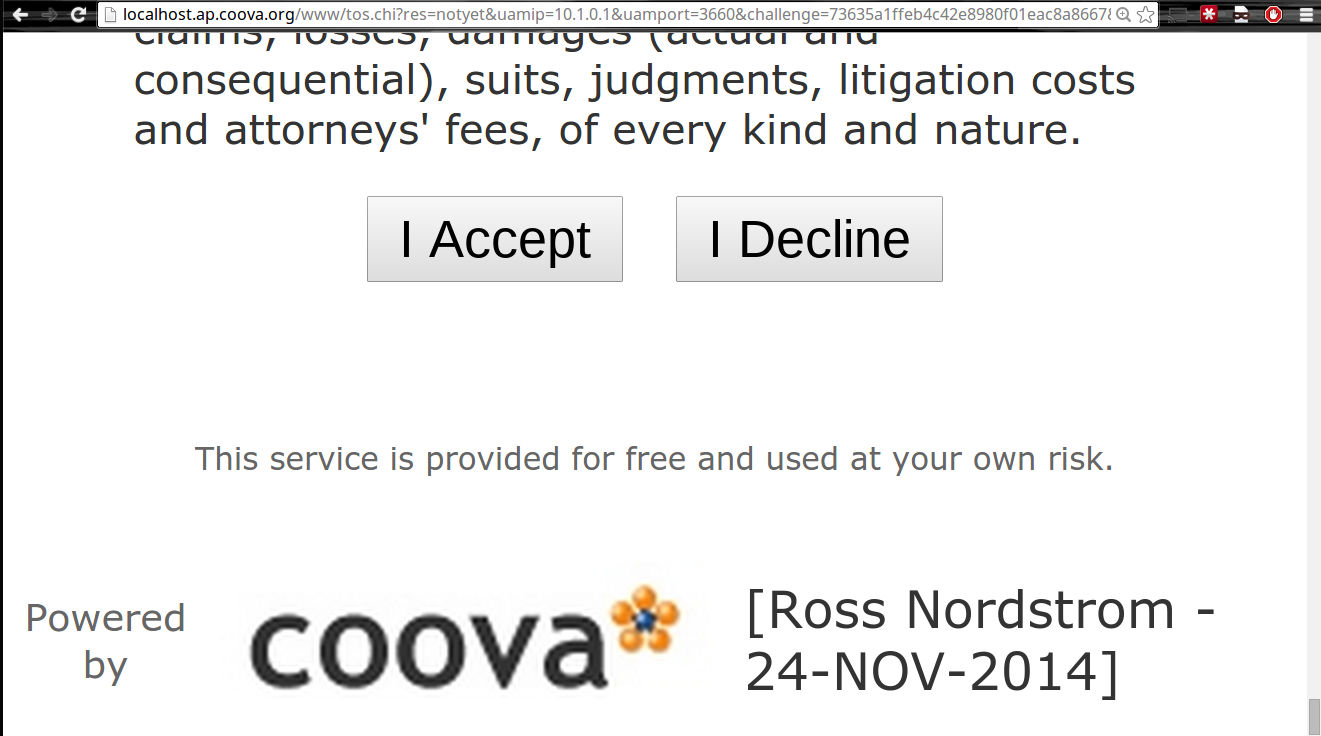
\includegraphics[width=90mm]{fig/footer.png}
\caption{Modified the Captive Portal!}
\label{fig:footer}
\end{figure}

\item{Explore:}  Next I tried to understand how the ToS page was served. Frighteningly, it seems to
be a served up by a Bash script. I managed to find the code driving the Footer and modify it to
include my name \ref{fig:footer}, by modifying a section of
\texttt{/etc/chilli/www/config-local.sh}.

\begin{figure}[ht!]
\centering
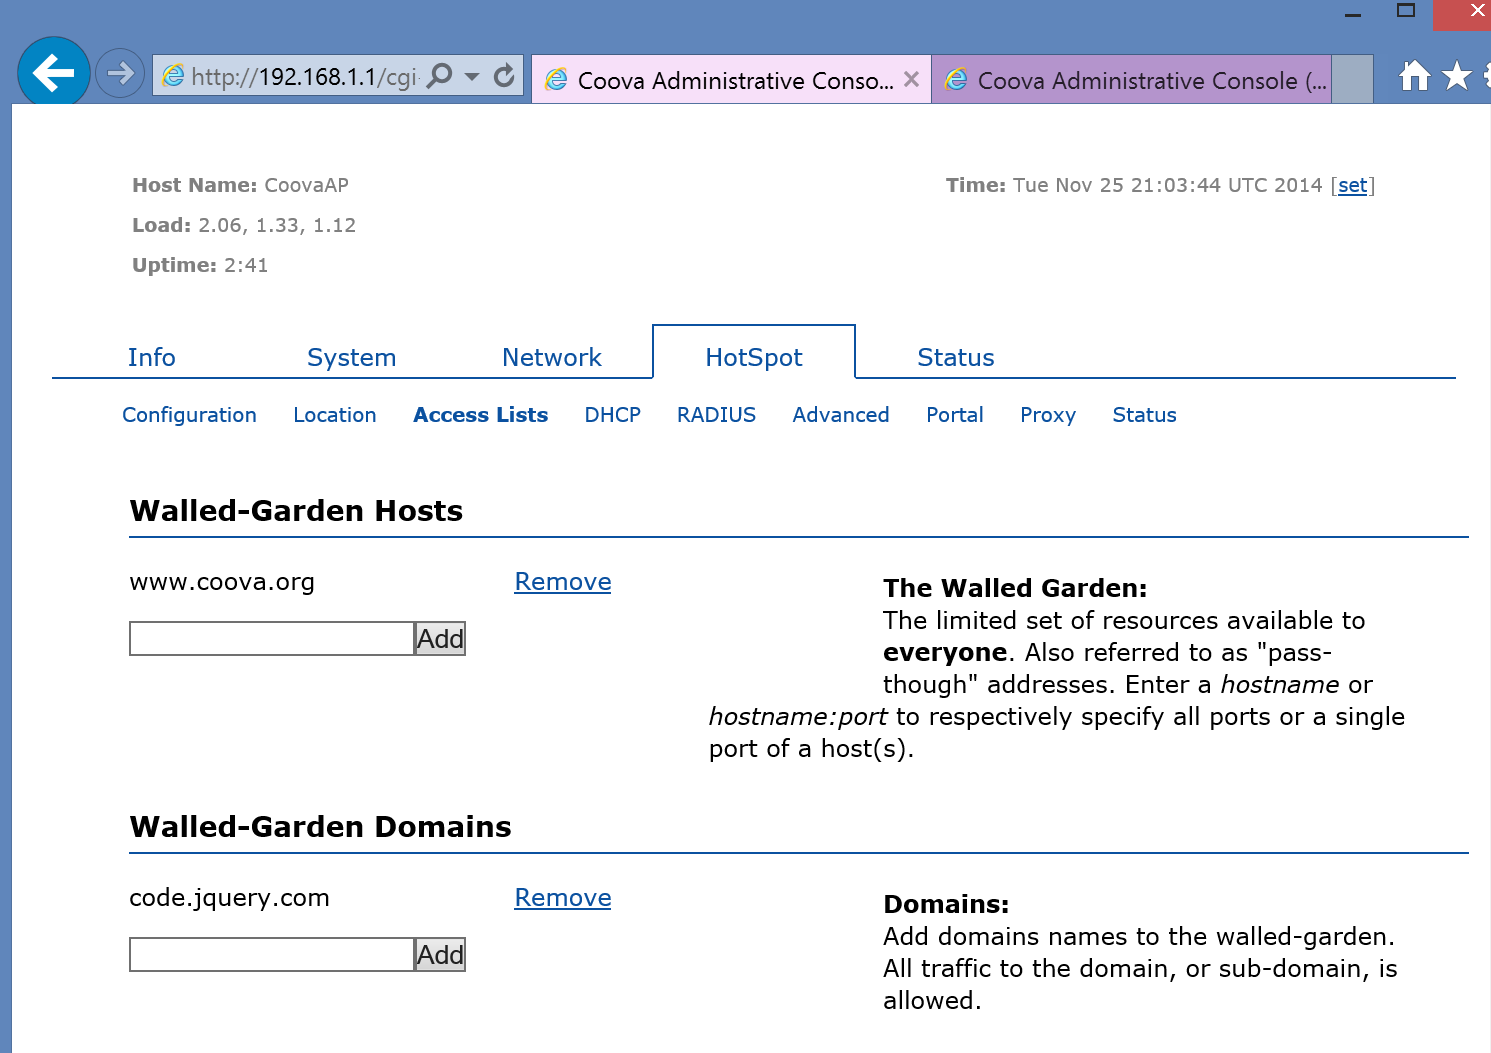
\includegraphics[width=90mm]{fig/allowed_domains1.png}
\caption{Allow jQuery within the Walled Garden}
\label{fig:allow_jquery}
\end{figure}

\begin{figure}[ht!]
\centering
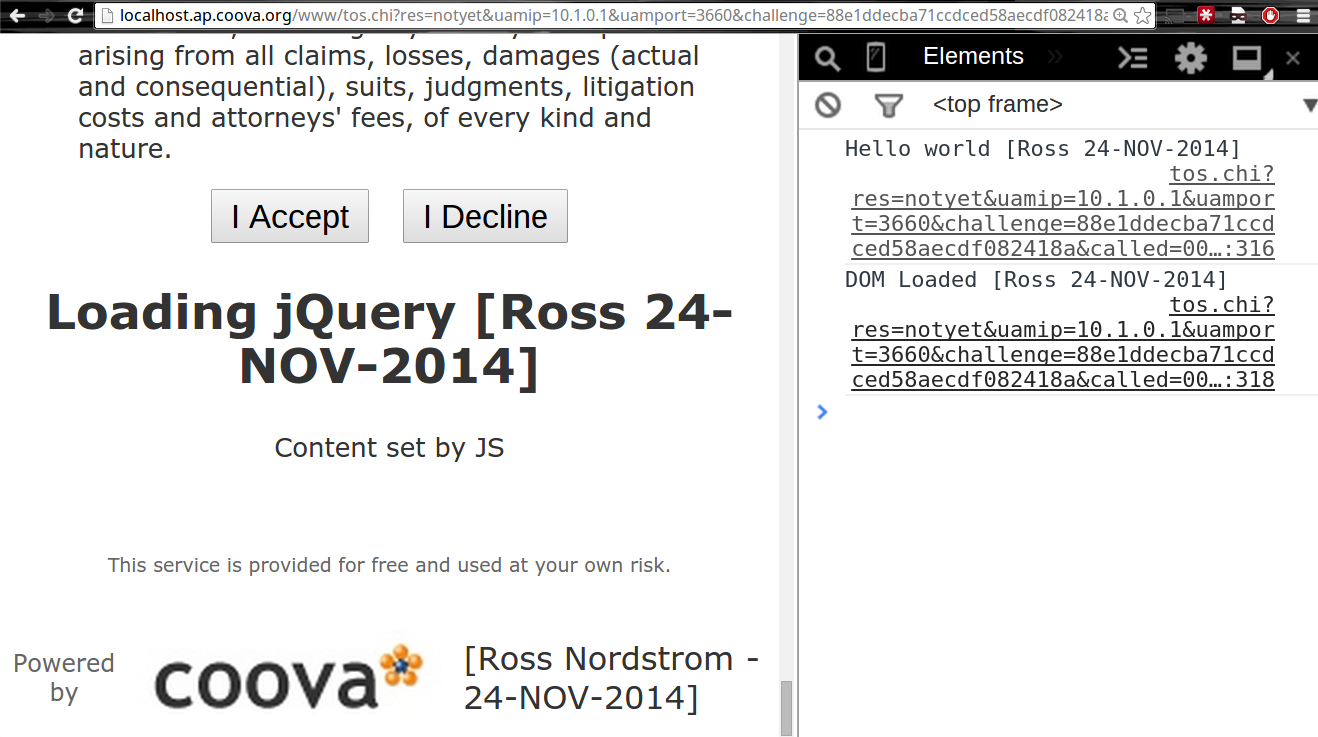
\includegraphics[width=90mm]{fig/jquery1.png}
\caption{and then use jQuery}
\label{fig:use_jquery}
\end{figure}

\item{Run jQuery:}  Knowing I could modify code, I next tried to run some custom JavaScript,
anticipating that I could use a JavaScript library to implement an OAuth client. To do this, I added
a \texttt{<script>} tag including \textunderscore{http\:\/\/code.jquery.com\/jquery-1.11.1.js}. This
of course didn't work initially because of the captive portal. To fix this, I added
``code.jquery.com'' to my allowed Domains in the Admin portal's Access List \ref{fig:allow_jquery}.
I was successfully able to use jQuery within the page then to overwrite a DOM element after page
load. The result is a console message and modified text \ref{fig:use_jquery}, having added some
JavaScript to the served page \cite{github:jquery}.

\begin{figure}[ht!]
\centering
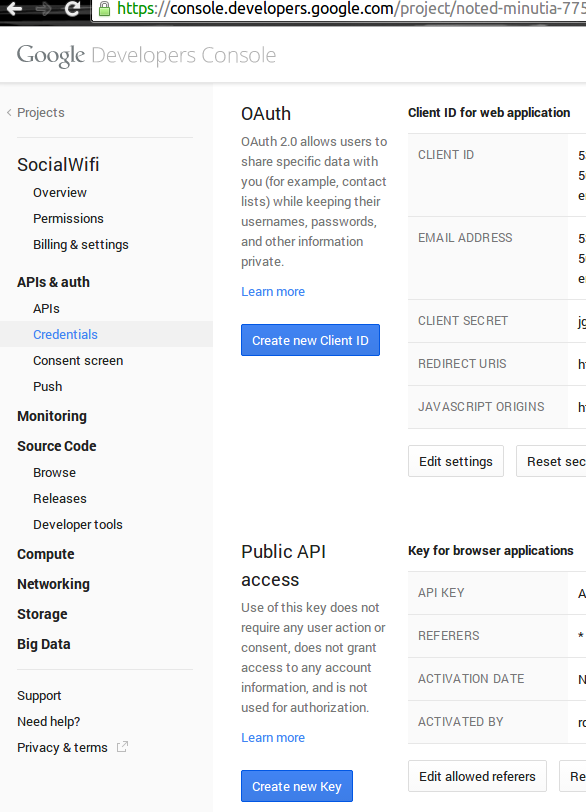
\includegraphics[width=90mm]{fig/google_project.png}
\caption{Google Project to authenticate against}
\label{fig:google_project}
\end{figure}

\item{Demo OAuth with Google:}  Now that I know I can run arbitrary JavaScript, I wanted to try
running the demonstration Google OAuth code \cite{google:OAuthDemo} from the router. To accomplish
this, I created a Google project \ref{fig:google_project} and configured a Client ID with which to
authenticate. An important step was to add ``localhost.ap.coova.org'' to the allowed referers and
JavaScript Origins fields.

\end{enumerate}

\end{document}

